\documentclass[12pt]{article}

\usepackage{amsmath}
\usepackage{amssymb}
\usepackage[pdftex]{graphicx}
\usepackage{multicol}

\date{September 2021}
\title{Optimisation with Progressive Sharpening}
\author{Sahil Trivedi}

\begin{document}
	\maketitle
	
	\begin{multicols}{2}
		
		\section{Abstract}
		Introducing Progressive Sharpening, a method for optimising convolutional and fully connected layers in neural networks. This is achieved by creating incrementally denoised (blurred) copies of the training data. Training is initialised with the most denoised samples, and every few epochs we progressively sharpen the samples until the network converges on the orginal training data. We discuss the mathematical intuition of our technique and benchmark it against SoTA models on image recognition datasets. 
		
		\section{Introduction}
		Gradient descent optimises the weights of a network by minimising the error for it's neurons' activation values. A common tradeoff associated with gradient descent is it's tendency to converge training around local minima. Despite extensive research in the area of learning rate optimisation, avoiding local minima remains a recurring challenge in deep learning.
		\\\\
		During denoising, high level features are preserved while obscure features are smoothened out of the data. This is leveraged early on during training as we want the network paramters to distinguish high level features and avoid lower level features associated with local minima. As training progresses and high level features are generalised, we proceed to increase the level of detail in our training data making the network focus on more obscure features towards the end of training.
		\\\\
		It is well established that vision in human infants is blurred and improves it's focus as time passes. We discuss the mathematical intuition behind progressive denoising in Section 6 of this paper.  
		
		\section{Network \\Architecture}
		Progressive Sharpening can potentially increase the accuracy of a model from moderately high to extremely high. For this to work we take a model with an acceptable accuracy/loss and make a few design changes based on our understanding of the problem domain along with some trial and error.
		\\\\
		In the context of Image Classification on the MNIST dataset, LeNet-5 is a popular architecture with consistently high performance. We modify LeNet-5 by adding dropout to it's dense layers. The model summary is given below.
		\\\\
		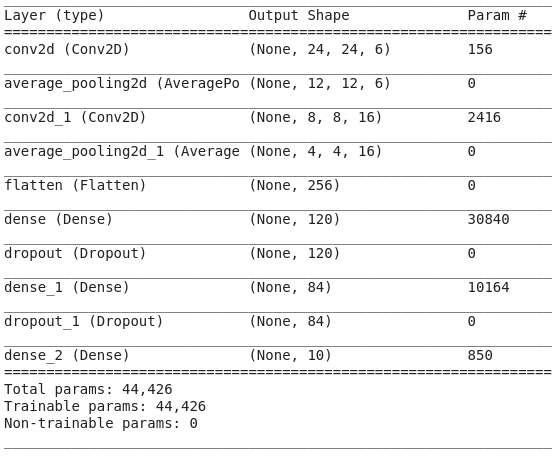
\includegraphics[width=\linewidth]{assets/summary.png}

		\section{Training}
		The specifics for implementing Progressive Sharpening largely depend on the problem domain. This paper implements the technique in context of Image Classification, but the principle extends for classifying information with any dimensional encoding.
		\subsection{Denoising Training Samples}
		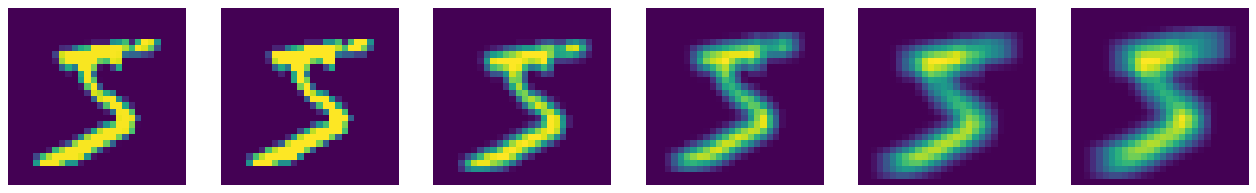
\includegraphics[width=\linewidth]{assets/denoise.png}
		\\\\
		The figure illustrates an original sample on the extreme left followed by it's progressively denoised copies. The original image is from the MNIST dataset and the denoising is carried out using low pass filters. The kernels for these filters are represented by the following matrices:
		$$ kernel_{N} = \frac{J_{N}}{N^2} $$
		where $J_{N}$ is an $N \times N$ matrix with all elements equal to $1$.
		\\\\
		Since $kernel_{1}$ denotes an identity transform, the first two images are identical and the latter four are progressively denoised. We apply the said convolutions to the training dataset which returns denoised copies of the training data. These copies are passed to the Convolutional Neural Network while training in a predetermined order.
		\subsection{Training Set \\Optimisation}
		The multiple sets of training data obtained from the previous step are referred to as $train_{1},train_{2}, \hdots ,train_{K}$ where 
		$$train_{n} = training\_data \circledast kernel_{n} $$
		and $K$ is equal to the denoising intervals picked for the data. $\circledast$ is a convolutional operator and the kernel denotes a low-pass filter for the training data. 
		\\\\
		The higher the value of $n$, the more denoised the data. We begin training with the most denoised copies of the training data. After few epochs we replace the training data with it's next most denoised copy. This process repeats $K$ times before network loss converges for the least denoised samples i.e. the original training data itself.
		
		\section{Benchmarking}
		
		\section{Mathematical \\Intuition}
		Gradient descent optimises the weights of a network by minimising the error in it's neurons' activation values. A common tradeoff associated with gradient descent is it's tendency to converge training around local minima. Learning Rate Optimisation is generally employed to address this.
		\\
		- Visualising W vs E hypersurface
		
	\end{multicols}

	\begin{multicols}{2}
		
	\end{multicols}
	
	
	
	
	
\end{document}
